\documentclass{article}

%%%%%%%%%%%%%%%%%%%%%%%%%%%%%%%%%%%%%%%%%
% Lachaise Assignment
% Structure Specification File
% Version 1.0 (26/6/2018)
%
% This template originates from:
% http://www.LaTeXTemplates.com
%
% Authors:
% Marion Lachaise & François Févotte
% Vel (vel@LaTeXTemplates.com)
%
% License:
% CC BY-NC-SA 3.0 (http://creativecommons.org/licenses/by-nc-sa/3.0/)
% 
%%%%%%%%%%%%%%%%%%%%%%%%%%%%%%%%%%%%%%%%%

%----------------------------------------------------------------------------------------
%	PACKAGES AND OTHER DOCUMENT CONFIGURATIONS
%----------------------------------------------------------------------------------------

\usepackage{amsmath,amsfonts,stmaryrd,amssymb} % Math packages

\usepackage{enumerate} % Custom item numbers for enumerations

\usepackage{url}

\usepackage[ruled]{algorithm2e} % Algorithms

\usepackage[framemethod=tikz]{mdframed} % Allows defining custom boxed/framed environments

\usepackage{listings} % File listings, with syntax highlighting
\lstset{
	basicstyle=\ttfamily, % Typeset listings in monospace font
}

\usepackage{indentfirst}
\setlength{\parindent}{2em}

%----------------------------------------------------------------------------------------
%	DOCUMENT MARGINS
%----------------------------------------------------------------------------------------

\usepackage{geometry} % Required for adjusting page dimensions and margins

\geometry{
	paper=a4paper, % Paper size, change to letterpaper for US letter size
	top=1.5cm, % Top margin
	bottom=2.5cm, % Bottom margin
	left=2.4cm, % Left margin
	right=2.4cm, % Right margin
	headheight=10pt, % Header height
	footskip=1.5cm, % Space from the bottom margin to the baseline of the footer
	headsep=1cm, % Space from the top margin to the baseline of the header
	% showframe, % Uncomment to show how the type block is set on the page
}

%----------------------------------------------------------------------------------------
%	FONTS
%----------------------------------------------------------------------------------------

\usepackage[utf8]{inputenc} % Required for inputting international characters
\usepackage[T1]{fontenc} % Output font encoding for international characters

% \usepackage{XCharter} % Use the XCharter fonts\usepackage{XCharter} % Use the XCharter fonts

%----------------------------------------------------------------------------------------
%	COMMAND LINE ENVIRONMENT
%----------------------------------------------------------------------------------------

% Usage:
% \begin{commandline}
%	\begin{verbatim}
%		$ ls
%		
%		Applications	Desktop	...
%	\end{verbatim}
% \end{commandline}

\mdfdefinestyle{commandline}{
	leftmargin=10pt,
	rightmargin=10pt,
	innerleftmargin=15pt,
	middlelinecolor=black!50!white,
	middlelinewidth=2pt,
	frametitlerule=false,
	backgroundcolor=black!5!white,
	frametitle={Command Line},
	frametitlefont={\normalfont\sffamily\color{white}\hspace{-1em}},
	frametitlebackgroundcolor=black!50!white,
	nobreak,
}

% Define a custom environment for command-line snapshots
\newenvironment{commandline}{
	\medskip
	\begin{mdframed}[style=commandline]
}{
	\end{mdframed}
	\medskip
}

%----------------------------------------------------------------------------------------
%	FILE CONTENTS ENVIRONMENT
%----------------------------------------------------------------------------------------

% Usage:
% \begin{file}[optional filename, defaults to "File"]
%	File contents, for example, with a listings environment
% \end{file}

\mdfdefinestyle{file}{
	innertopmargin=1.6\baselineskip,
	innerbottommargin=0.8\baselineskip,
	topline=false, bottomline=false,
	leftline=false, rightline=false,
	leftmargin=1cm,
	rightmargin=1cm,
	singleextra={%
		\draw[fill=black!10!white](P)++(0,-1.2em)rectangle(P-|O);
		\node[anchor=north west]
		at(P-|O){\ttfamily\mdfilename};
		%
		\def\l{3em}
		\draw(O-|P)++(-\l,0)--++(\l,\l)--(P)--(P-|O)--(O)--cycle;
		\draw(O-|P)++(-\l,0)--++(0,\l)--++(\l,0);
	},
	nobreak,
}

% Define a custom environment for file contents
\newenvironment{file}[1][File]{ % Set the default filename to "File"
	\medskip
	\newcommand{\mdfilename}{#1}
	\begin{mdframed}[style=file]
}{
	\end{mdframed}
	\medskip
}

%----------------------------------------------------------------------------------------
%	NUMBERED QUESTIONS ENVIRONMENT
%----------------------------------------------------------------------------------------

% Usage:
% \begin{question}[optional title]
%	Question contents
% \end{question}

\mdfdefinestyle{question}{
	innertopmargin=1.2\baselineskip,
	innerbottommargin=0.8\baselineskip,
	roundcorner=5pt,
	nobreak,
	singleextra={%
		\draw(P-|O)node[xshift=1em,anchor=west,fill=white,draw,rounded corners=5pt]{%
		Question \theQuestion\questionTitle};
	},
}

\newcounter{Question} % Stores the current question number that gets iterated with each new question

% Define a custom environment for numbered questions
\newenvironment{question}[1][\unskip]{
	\bigskip
	\stepcounter{Question}
	\newcommand{\questionTitle}{~#1}
	\begin{mdframed}[style=question]
}{
	\end{mdframed}
	\medskip
}

%----------------------------------------------------------------------------------------
%	WARNING TEXT ENVIRONMENT
%----------------------------------------------------------------------------------------

% Usage:
% \begin{warn}[optional title, defaults to "Warning:"]
%	Contents
% \end{warn}

\mdfdefinestyle{warning}{
	topline=false, bottomline=false,
	leftline=false, rightline=false,
	nobreak,
	singleextra={%
		\draw(P-|O)++(-0.5em,0)node(tmp1){};
		\draw(P-|O)++(0.5em,0)node(tmp2){};
		\fill[black,rotate around={45:(P-|O)}](tmp1)rectangle(tmp2);
		\node at(P-|O){\color{white}\scriptsize\bf !};
		\draw[very thick](P-|O)++(0,-1em)--(O);%--(O-|P);
	}
}

% Define a custom environment for warning text
\newenvironment{warn}[1][Warning:]{ % Set the default warning to "Warning:"
	\medskip
	\begin{mdframed}[style=warning]
		\noindent{\textbf{#1}}
}{
	\end{mdframed}
}

%----------------------------------------------------------------------------------------
%	INFORMATION ENVIRONMENT
%----------------------------------------------------------------------------------------

% Usage:
% \begin{info}[optional title, defaults to "Info:"]
% 	contents
% 	\end{info}

\mdfdefinestyle{info}{%
	topline=false, bottomline=false,
	leftline=false, rightline=false,
	nobreak,
	singleextra={%
		\fill[black](P-|O)circle[radius=0.4em];
		\node at(P-|O){\color{white}\scriptsize\bf i};
		\draw[very thick](P-|O)++(0,-0.8em)--(O);%--(O-|P);
	}
}

% Define a custom environment for information
\newenvironment{info}[1][Info:]{ % Set the default title to "Info:"
	\medskip
	\begin{mdframed}[style=info]
		\noindent{\textbf{#1}}
}{
	\end{mdframed}
}


\usepackage{fontspec}
\usepackage{multicol}
\usepackage{enumitem}
\usepackage{url}
\usepackage{booktabs} 

\XeTeXlinebreaklocale "zh"
\XeTeXlinebreakskip = 0pt plus 1pt
\setmainfont{Noto Sans CJK KR}

\title{高级计算机视觉实验报告}

\author{张义飞}

\date{201821080630}

\begin{document}

\maketitle

\section{图像混合}
\begin{question}
    本项目要求使用高斯滤波实现图像混合,具体要求为:
    \begin{enumerate}
        \item 手动实现滤波器;
        \item 使用高斯滤波提取两张图片的低频与高频信息,并将之混合。
    \end{enumerate}
\end{question}

\subsection{项目细节}
滤波器函数主要包含以下几个部分:
\begin{enumerate}
    \item 图像预处理,如果输入图片是灰度图,提升图片最后一维,使其结构与RGB图保持一致,此举是为了同时兼容灰度图和RGB彩色图;
    \item 图片填充(padding),分别获取图片长宽与滤波器长宽,然后计算图片的填充值,首先根据滤波操作的输出尺寸公式:
    \begin{equation}
        I_{out}=\frac{I_{in}-K_{size}+L_{padding}+R_{padding}}{step}+1
    \end{equation}
    本实验中的$step=1$,令$I_{out}=I_{in}$,得:
    \begin{equation}
        L_{padding}+R_{padding}=\frac{K_{size}-1}{2}
    \end{equation}
    在代码实现中,使用以下逻辑生成填充范围:
    \begin{eqnarray}
        D=(K_{size}-1)\ mod\ 2 \\
        L_{padding}=\frac{K_{size}-1-D}{2} \\
        R_{padding}=\frac{K_{size}-1+D}{2}
    \end{eqnarray}
    \item 滤波运算(卷积),对图片的每个通道上的矩阵进行分块计算,获得滤波后的图片输出。
\end{enumerate}

\begin{figure}[h]
    \centering
    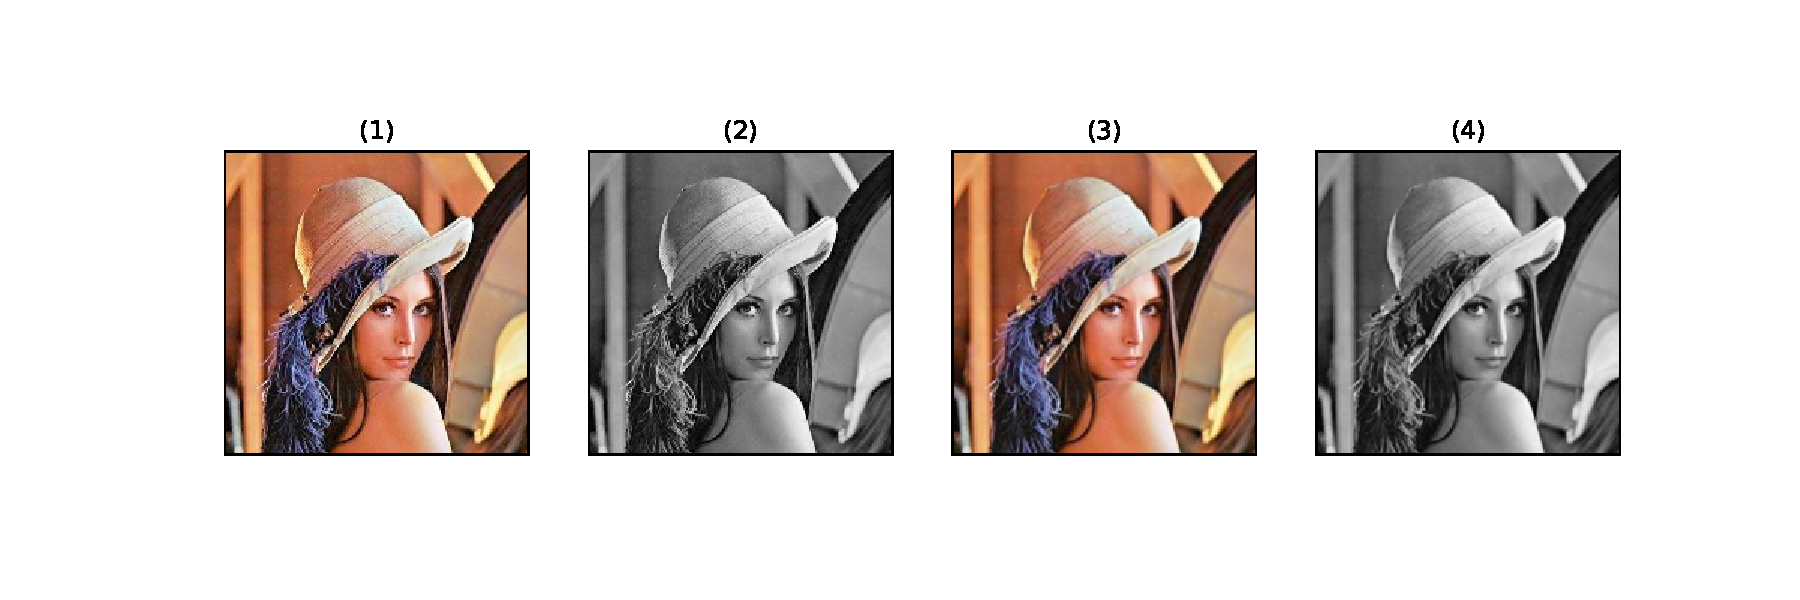
\includegraphics[width=\textwidth]{./project1/img/filter.pdf}
    \caption{滤波器函数输出示例,其中(1)和(2)为彩色以及灰度原图,(3)(4)分别为彩色和灰度图进行了$3\times 3$均值滤波后的处理图。}
\end{figure}

得到图片滤波函数之后,需要计算出对应尺寸的高斯滤波算子,用来提取图片中低频以及高频部分,根据高斯滤波函数的定义:
\begin{equation}
    G_\sigma = \frac{1}{2\pi \sigma}e^{-\frac{x^2+y^2}{2\sigma ^2}}
\end{equation}
对应的代码实现:
\begin{lstlisting}[language=Python, frame=shadowbox]
def gaussianKernel(sigma, n=2):
    size = n * sigma + 1
    kernel = np.zeros((size, size))
    center = size / 2
    for x in range(size):
        for y in range(size):
            kernel[x, y] = np.exp(-0.5 * (x * x + y * y) / 2 / sigma / sigma)
    return kernel / np.sum(kernel)
\end{lstlisting}

\begin{figure}[h]
    \centering
    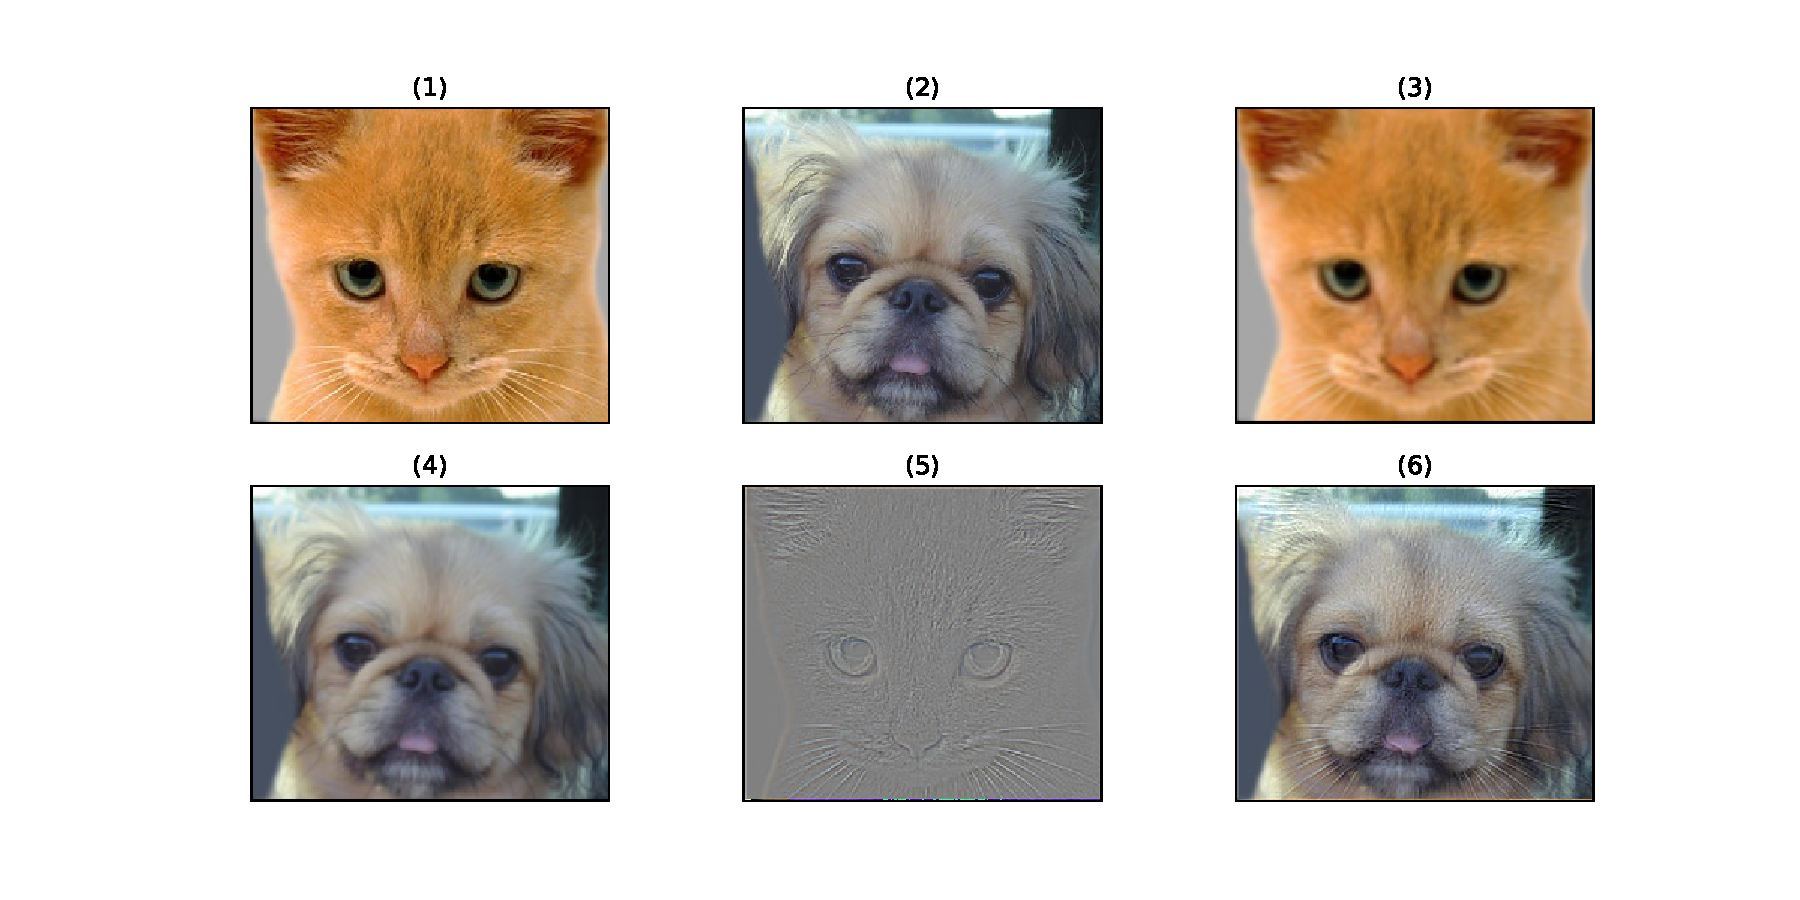
\includegraphics[width=\textwidth]{./project1/img/hybird.pdf}
    \caption{图像混合结果,其中(1)(2)为混合图像原图,(3)(4)为高斯滤波结果,(5)为图(2)高频部分,(6)为图片混合结果。}
\end{figure}

\subsection{核心代码}
\begin{lstlisting}[language=Python, frame=shadowbox]
import numpy as np

"""
图片滤波器

自动padding,输出卷积后的图像
"""
def imfilter(im:list, kernel:list, step=1)->list:
    src_img = np.array(im)
    kernel = np.array(kernel)

    im = src_img

    # 将灰度图与彩色图像保持一致
    if len(im.shape) == 2:
        im = im.reshape(im.shape + (1, ))

    # 分别取图像宽高和滤波器宽高
    [ih, iw] = im.shape[0:2]
    [kh, kw] = kernel.shape[0:2]
    
    # 不合法的输入
    if iw < kw or ih < kh:
        return None

    # 计算padding值
    wp = getPad(kw - 1)
    hp = getPad(kh - 1)

    # padding
    pimg = np.pad(im, (hp, wp, (0, 0)), 'constant', constant_values=(0, 0))

    # 变换,将像素拆分成R, G, B各通道的图片
    pimg = pimg.transpose()

    # 设定输出值,输出矩阵与输入矩阵保持一致
    ret_img = np.zeros(im.shape[::-1])

    # 获取padding后的图像宽高
    [channel, ph, pw] = pimg.shape

    # 执行滤波,对每一个通道都进行处理
    for chn in range(channel):
        for r in range(0, ph - kh):
            for c in range(0, pw - kw):
                ret_img[chn, r, c] = np.sum(pimg[chn, r:r + kh, c:c + kw] * \
                    kernel)

    # 结果转置为RGB图像
    ret_img = ret_img.transpose()
    if ret_img.shape[-1] == 1:
        ret_img = ret_img.reshape(ret_img.shape[0:2])

    return ret_img.astype(np.uint8)

def getPad(dis:int)->tuple:
    dis = 0 if dis < 0 else dis
    return ((dis - dis % 2) // 2, (dis + dis % 2) // 2)
\end{lstlisting}

\begin{lstlisting}[language=Python, frame=shadowbox]
def hybird():
    cat_img = imread('cat.jpg')
    dog_img = imread('dog.jpg')

    cat_kernel = gaussianKernel(3)
    dog_kernel = gaussianKernel(2)

    cat_blur = imfilter(cat_img, cat_kernel)
    dog_blur = imfilter(dog_img, dog_kernel)

    # 需要临时扩展
    cat_high = cat_img.astype(np.int16) - cat_blur.astype(np.int16)

    hybird_img = cat_high + dog_blur
    plt.figure(figsize=(12, 6))

    imgs = [cat_img, dog_img, cat_blur, dog_blur, cat_high, hybird_img]
    for index, img in enumerate(imgs):
        plt.subplot(1, len(imgs), index + 1)
        # img = cv2.cvtColor(img, cv2.COLOR_RGB2BGR)
        plt.imshow(img)
        plt.xticks([])
        plt.yticks([])
        plt.title('(%d)' % (index + 1))

    plt.savefig(FILE_PATH + 'hybird.pdf')
\end{lstlisting}

\section{局部特征匹配}
\begin{question}
    本实验通过对两张图片进行特征点检测、特征描述、特征匹配等系列操作,对两张图片进行特征点匹配,主要包含以下内容:
    \begin{enumerate}
        \item 实现Harris角点检测算法;
        \item 实现SIFT特征算子算法;
        \item 实现特征匹配。
    \end{enumerate}
\end{question}

\subsection{项目细节}
\subsubsection{Harris角点检测}
角点检测是计算机视觉系统中用来提取图像特征的一种方法,又称为特征点检测。被广泛用于运动检测,图像匹配,视频跟踪,三维建模和目标识别等任务中。角点通常被定义为两条边的交点,更严格的说,角点的局部邻域应该具有两个不同区域的不同方向的边界。

而实际应用中,大多数所谓的角点检测方法检测的是拥有特定特征的图像点,而不仅仅是“角点”。这些特征点在图像中有具体的坐标,并具有某
些数学特征,如局部最大或最小灰度、某些梯度特征等。角点检测领域一个著名的算法就是Harris角点检测算法。眼对角点的识别通常是在一个局部的小区域或小窗口完成的。如果在各个方向上移动这个特征的小窗口,窗口内区域的灰度发生了较大的变化,那么就认为在窗口内遇到了角点。如果这个特定的窗口在图像各个方向上移动时,窗口内图像的灰度没有发生变化,那么窗口内就不存在角点;如果窗口在某一个方向移动时,窗口内图像的灰度发生了较大的变化,而在另一些方向上没有发生变化,那么,窗口内的图像可能就是一条直线的线段。

对于图像$I(x,y)$,点$(x,y)$平移$(\Delta x,\Delta y)$后的自相似性,可以通过自相关函数给出:
\begin{equation}
    c(x, y; \Delta x, \Delta y)=\sum_{(u,v)\in W(x,y)}w(u,v)(I(x,y)-I(x+\Delta x, y+\Delta y))^2
    \label{self-eq}
\end{equation}

其中$W(x,y)$是$(x,y)$处的窗口,$w(x,y)$为加权函数。对(\ref{self-eq})式进行一阶近似:
\begin{equation}
    I(x+\Delta x, y+\Delta y)\approx I(x,y)+I_x(x,y)\Delta x+I_y(x,y)\Delta y
\end{equation}

也就是说图像$I(x,y)$在点$(x,y)$处平移$(\Delta x, \Delta y)$后的自相关函数可以近似为而像函数如:
		
\begin{equation}
c(x,y; \Delta x, \Delta y) \approx A\Delta x^2 + 2C\Delta x \Delta y + B\Delta y^2
\end{equation}
其中:
\begin{equation}
A=\sum_{w}I_{x}^{2}, B=\sum_{w}I_{y}{2}, C=\sum_{w}I_{x}I_{y}
\end{equation}
\begin{equation}
M(x,y)=\left[ \begin{array}{ccc}
A & C \\
C & B \\
\end{array} 
\right ]
\end{equation}
Harris角点检测的响应值:
\begin{equation}
R=detM-\alpha (traceM)^2
\end{equation}
通过Harris角点检测提出的响应值R,并且对小于某一阈值t的R置为0,之后在某个邻域内进行非极大值抑制,局部最大值点即为图中的角点。

\subsubsection{SIFT特征描述子}
Sift提取图像的局部特征,在尺度空间寻找极值点,并提取出其位置、尺度、方向信息。Sfit的应用范围包括物体辨别、机器人地图感知与导航、影响拼接、3D模型建立、手势识别、影响追踪等。
首先SIFT有下面几大特点:
\begin{enumerate}
    \item 对旋转、尺度缩放、亮度变化保持不变性,对视角变化、噪声等也存在一定程度的稳定性;
    \item 独特性,信息量丰富,适用于在海量特征数据中进行快速,准确的匹配;
    \item 多量性,即使少数几个物体也可以产生大量的Sfit特征向量;
    \item 可扩展性,可以很方便的与其他形式的特征向量进行联合;
\end{enumerate}
SIFT算法的实质是在不同的尺度空间上查找关键点(特征点),计算关键点的大小、方向、尺度信息,利用这些信息组成关键点对特征点进行描述的问题。SIFT所查找的关键点都是一些十分突出,不会因光照,仿射便函和噪声等因素而变换的“稳定”特征点,如角点、边缘点、暗区的亮点以及亮区的暗点等。

\begin{figure}[h]
    \centering
    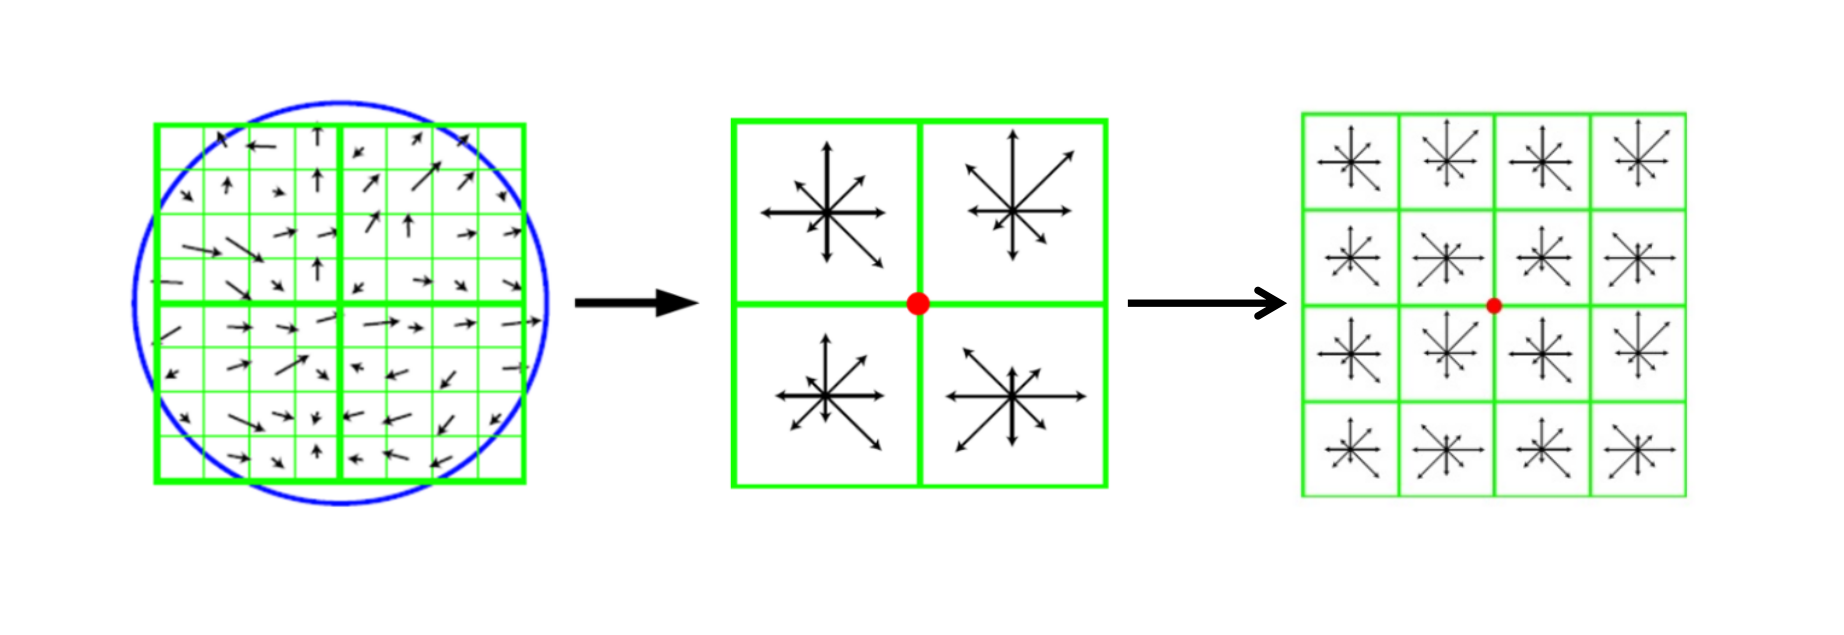
\includegraphics[width=\textwidth]{./project2/SIFT.png}
    \caption{从图像中产生SIFT描述子}
\end{figure}

SIFT的主要为了下面几个步骤:
\begin{enumerate}
	\item 生成高斯差分金字塔(DOG金字塔),尺度空间构建
	\item 空间极值点检测(关键点的初步查探)
	\item  稳定关键点的精确定位
	\item 稳定关键点方向信息分配
	\item 关键点描述
	\item  特征点匹配
\end{enumerate}
其中在关键点描述,产生描述子是后续实现匹配的关键步骤,描述其实就是一种以数学方式定义关键的过程。描述子不但包含关键点,也包括关键点周围对其有贡献的邻域点。描述的思路是:对关键点周围像素区域分块,计算快内梯度直方图,生成具有独特性的向量,这个向量是该区域图像信息的一种抽象表述。如下图,对于$4\times 4$块,每块的所有像素点的荼毒做高斯加权,每块最终取8个方向,即可以生成$4\times 4\times 8$维度的向量,以这$2\times 2\times 8$维向量作为中心关键点的数学描述。

\begin{figure}[h]
    \centering
    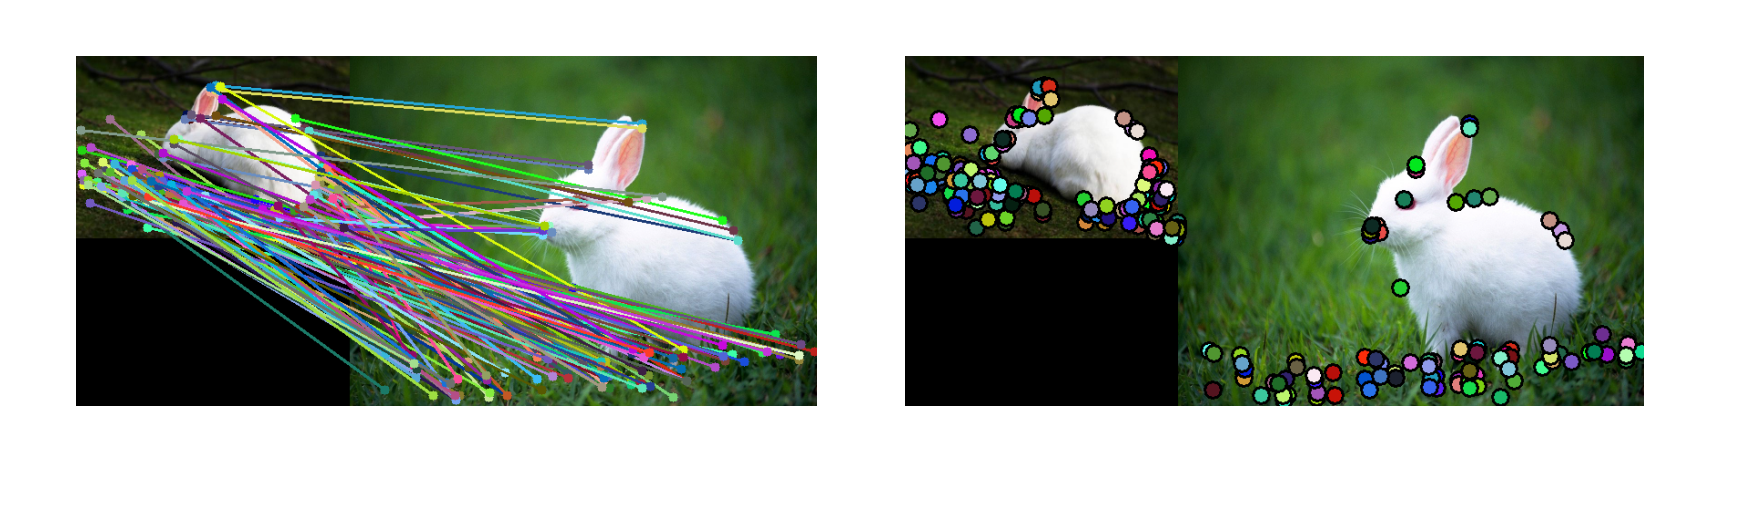
\includegraphics[width=\textwidth]{./project2/feature-match.png}
    \caption{特征匹配结果}
\end{figure}

\subsection{核心代码}
\begin{lstlisting}[language=Python]

def get_interest_points(image, feature_width):
    h, w = image.shape[:2]
    # TODO Write harrisdetector function based on the illustration in specification.
    # Return corner points x-coordinates in result[0] and y-coordinates in result[1]
    image = image.astype(float)

    print('Start getting image interest points\n')

    k = 4  # change to your value
    t = 0.35  # change to your value

    image = np.pad(image, (k, k), 'edge')
    # Laplace gradient kernal
    x_dev_kernal = np.array([[0, 0, 0], [-1, 0, 1], [0, 0, 0]])
    y_dev_kernal = np.array([[0, -1, 0], [0, 0, 0], [0, 1, 0]])
    # Laplace gradient
    x_dev = cv2.filter2D(image, -1, x_dev_kernal)
    y_dev = cv2.filter2D(image, -1, y_dev_kernal)

    Ixx = x_dev ** 2
    Iyy = y_dev ** 2
    IxIy = x_dev * y_dev

    eigen_values_map = np.zeros_like(image)
    for i_x in range(k, h + k):
        for i_y in range(k, w + k):
            A11 = Ixx[i_x - k:i_x + k + 1, i_y - k:i_y + k + 1]
            A21 = IxIy[i_x - k:i_x + k + 1, i_y - k:i_y + k + 1]
            A22 = Iyy[i_x - k:i_x + k + 1, i_y - k:i_y + k + 1]

            A11 = A11.sum()
            A21 = A21.sum()
            A22 = A22.sum()

            A = np.array([[A11, A21], [A21, A22]], dtype=np.float32)
            ret, eigenvalues, eigen_vector = cv2.eigen(A, False)
            if abs(eigenvalues[0]) > t and abs(eigenvalues[1]) > t:
                eigen_values_map[i_x, i_y] = eigenvalues[0] * eigenvalues[1]

    eigen_values_map = eigen_values_map[k:k + h, k:k + w]
    # local max
    r = 5
    for i in range(h - r):
        for j in range(w - r):
            window = eigen_values_map[i:i + r, j:j + r]
            if window.sum() == 0:
                continue
            else:
                local_max = np.max(window)
            # zero all but the localMax in the window
            max_x, max_y = (window == local_max).nonzero()
            window[:] = 0
            window[max_x, max_y] = local_max
            eigen_values_map[i:i + r, j:j + r] = window

    x, y = (eigen_values_map > 0).nonzero()
    x = x.reshape(len(x), 1)
    y = y.reshape(len(y), 1)

    print('Done\n')
    return y, x


def get_features(image, x, y, feature_width):


    print('Starting get features\n')
    # Placeholder that you can delete. Empty features.
    features = np.zeros((x.shape[0], 128))
    x_ = x.astype(int)
    y_ = y.astype(int)
    y = np.squeeze(x_)
    x = np.squeeze(y_)
    h, w = image.shape[:2]
    # pad to avoid 0
    offset = int(feature_width / 2)
    image = np.pad(image, (offset, offset), 'edge')
    x += offset
    y += offset

    # step 1 Gaussian blur whole image
    k = 7
    blur_image = cv2.GaussianBlur(image, (k, k), sigmaX=0)  # kernal size is changable, 19 is best 69.8%

    # step 2 gradients
    x_kernal = np.array([[-1, 1]])
    Gx = cv2.filter2D(blur_image, -1, x_kernal)
    Gy = cv2.filter2D(blur_image, -1, np.transpose(x_kernal))

    # step 3 magnitude and orientation
    mag = np.sqrt(Gx ** 2 + Gy ** 2)
    orient = np.arctan2(Gy, Gx)
    orient[orient < 0] += np.pi * 2

    # step 4 further weighted by Gaussian
    cell_length = feature_width / 4
    Gau_kernel = cv2.getGaussianKernel(feature_width, feature_width / 2)

    for i in range(x.shape[0]):
        w = int(feature_width / 2)
        window = mag[(x[i] - w):(x[i] + w),
                    (y[i] - w):(y[i] + w)]
        window = cv2.sepFilter2D(window, -1, Gau_kernel, np.transpose(Gau_kernel))
        window_orient = orient[(x[i] - w):(x[i] + w),
                        (y[i] - w):(y[i] + w)]
        for i_x in range(4):
            for i_y in range(4):
                bin = np.zeros(8)
                cell = window[int(i_x * cell_length):int((i_x + 1) * cell_length), int(i_y * cell_length):int((i_y + 1) * cell_length)]
                cell_orient = window_orient[int(i_x * cell_length):int((i_x + 1) * cell_length),
                                int(i_y) * int(cell_length):int((i_y + 1)) * int(cell_length)]
                for angle in range(bin.shape[0]):
                    bin[angle] += np.sum(
                        cell[np.all([cell_orient >= (angle * np.pi / 4), cell_orient < ((angle + 1) * np.pi / 4)], 0)])
                features[i, (i_x * 4 + i_y) * 8:(i_x * 4 + i_y) * 8 + 8] = bin
        # step 6 normalization
        features[i, :] /= np.sqrt(np.sum(features[i, :] ** 2))

    print('Done\n')
    return features


def match_features(features1, features2, threshold=0.0):

    print('Starting matching features\n')
    # Placeholder that you can delete. Random matches and confidences
    num_features = max(features1.shape[0], features2.shape[0])
    matched = np.zeros((num_features, 2))
    confidence = np.zeros((num_features, 1))

    for i in range(features1.shape[0]):
        dist = np.sqrt(np.sum((features1[i] - features2) ** 2, axis=1))  # (n2,k)->n2
        smallest = np.min(dist)
        second_smallest = np.partition(dist, 1)[1]
        ratio = smallest / second_smallest
        confidence[i] = 1 / ratio
        matched[i, 0] = i
        matched[i, 1] = np.argmin(dist)

    # Sort the matches so that the most confident onces are at the top of the
    # list. You should probably not delete this, so that the evaluation
    # functions can be run on the top matches easily.
    order = np.argsort(confidence, axis=0)[::-1, 0]
    confidence = confidence[order, :]
    matched = matched[order, :]

    # delete the ones not so confident
    index_x, index_y = (confidence > threshold).nonzero()
    confidence = confidence[index_x, index_y]
    matched = matched[index_x, :]

    print('Done\n')
    return matched, confidence


def cheat_interest_points(eval_file, scale_factor):
    data = np.load(eval_file).tolist()
    x1 = data['x1']
    y1 = data['y1']
    x2 = data['x2']
    y2 = data['y2']
    x1 = x1 * scale_factor
    y1 = y1 * scale_factor
    x2 = x2 * scale_factor
    y2 = y2 * scale_factor

    return x1, y1, x2, y2  # they are float...


def show_correspondence(imgA, imgB, X1, Y1, X2, Y2, file_name='result'):
    Height = max(imgA.shape[0], imgB.shape[0])
    Width = imgA.shape[1] + imgB.shape[1]
    if len(imgA.shape) == 2:
        imgA = np.expand_dims(imgA, 2)
    if len(imgB.shape) == 2:
        imgB = np.expand_dims(imgB, 2)
    numColors = imgA.shape[2]
    newImg = np.zeros((Height, Width, numColors))
    newImg[:imgA.shape[0], :imgA.shape[1], :] = imgA
    newImg[:imgB.shape[0], imgA.shape[1]:, :] = imgB
    shiftX = imgA.shape[1]
    for i in range(X1.shape[0]):
        cur_color = np.random.rand(3)
        cv2.circle(newImg, (X1[i], Y1[i]), 9, cur_color, -1)
        cv2.circle(newImg, (X1[i], Y1[i]), 9, [0, 0, 0], 2)
        cv2.circle(newImg, (X2[i] + shiftX, Y2[i]), 9, cur_color, -1)
        cv2.circle(newImg, (X2[i] + shiftX, Y2[i]), 9, [0, 0, 0], 2)

    print('Saving visualization to vis_dots_' + file_name + '.png')
    cv2.imwrite('vis_dots_' + file_name + '.png', newImg * 255.0)
\end{lstlisting}

\section{词袋模型实现场景识别}
\subsection{项目细节}
词袋模型(Bag of Words, BOW)最初被用在文本分类中。它的基本思想是假定对于一个文本,忽略其词汇顺序、语法、句法,仅将其看作是一些词汇的集合,而文本里的每个词汇都是独立的,用词汇的出现频率来代表整个句子的含义。在此基础上,有学者提出视觉词袋模型。即将一幅图像看作是一些主题对象(视觉词汇)的集合,以视觉词汇出现的频率作为图像的特征进行识别和分类。Bag-of-words在CV中的应用首先出现在Andrew Zisserman中为解决对视频场景的搜索,其提出了使用Bag-of-words关键点投影的方法来表示图像信息。后续更多的研究者归结此方法为Bag-of-Features,并用于图像分类、目标识别和图像检索。Bag-of-Features模型仿照文本检索领域的Bag-of-Words方法,把每幅图像描述为一个局部区域或关键点(Patches/Key Points)特征的无序集合,这些特征点可以看成一个词。这样,就能够把文本检索及分类的方法用到图像分类及检索中去。

\begin{question}
    典型的词袋特征算法实现场景识别,应当包括以下几个步骤:
    \begin{enumerate}
        \item 对于一个场景影像数据集,从中随机选取足够数量的小块,提取特征作为视觉词汇;
        \item 然后经过字典学习之后形成场景词汇字典;对要一个待分类的场景图片,将其分割成若干个影像块,提取影像块特征;
        \item 根据字典对各个影像块进行编码;进行池化之后得到影像的词汇频率,作为影像的特征向量;
        \item 根据得到的向量对影像进行分类,得到所属类别。
    \end{enumerate}
\end{question}

\begin{figure}[h]
    \centering
    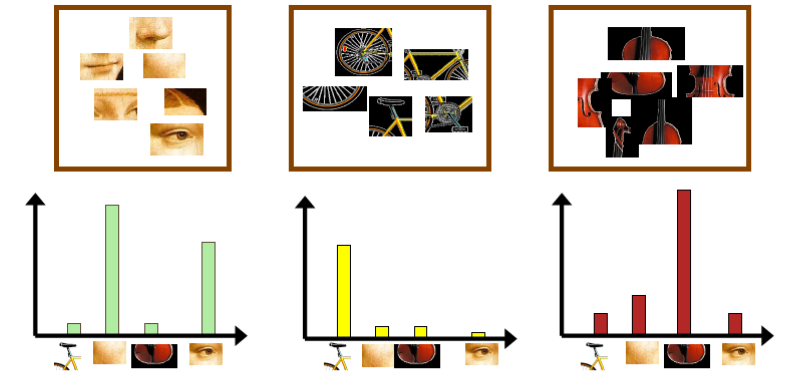
\includegraphics[width=\textwidth]{./project3/bow.png}
    \caption{词袋特征算法中,使用视觉词汇的频率表示图片特征。}
\end{figure}

\subsubsection{特征提取}
特征的提取方法有很多,实验中主要涉及到的有三种:原始像素特征(RAW),均值和标准差特征(MSTD),稠密SIFT特征(Dense SIFT)。原始像素特征是最常见和底层的描述图像特征的方式,方法就是将图像所有像素逐行,逐列或逐波段排列成一个列向量,作为图像的代表向量。假设图像块的大小为 $m * n$ ,包含 $p$ 个波段,那么该图像块的代表向量的大小就是 $(m * n * p, 1)$。均值和标准差特征也是一种常见且比较简单的特征,它是求出影像块各个波段均值和标准差,排列成一个向量,作为影像块的代表。向量的大小就是 $(2 * p, 1)$。SIFT特征具有尺度不变性的优点,可以在图像中检测出关键点,是一种局部特征描述子。而Dense SIFT特征是在SIFT基础上的改进,研究表明,Dense SIFT特征在目标分类和场景识别等领域的效果比SIFT要好。对于每一个图像块,Dense SIFT通过计算 $4\times 4$ 个互不覆盖的字块在8个方向上的的局部直方图来获得描述向量,描述向量的大小就是 $(128, 1)$。对影像的每个波段都提取Dense SIFT特征,因此每个影像块特征的大小就是 $(128, p)$。

\subsubsection{建立视觉字典}
视觉词汇的字典学习也是一个非常重要的过程。得到的字典一般要求具有完备性和代表性,这就要求在选取影像块的时候要随机选择足够多的影像块,并且字典的规模要控制在合适的范围之内。具体而言,首先从场景影像数据集中随机选择大量的影像块,例如选择100000个随机影像块作为原数据提取特征;然后利用聚类的方法形成字典,常用的做法是Kmeans聚类,例如聚成1000类,得到1000个聚类中心作为字典素材。此外,在聚类之前,会对提取到的特征进行预处理,例如ZCA白化和标准化来消除特征的各个维度之间的相关性,提高字典学习的效果。

\subsubsection{视觉特征的量化表示}
在得到字典之后,就可以对于一个场景图片进行特征编码,获得其编码表达。对于一幅场景影像,获取影像块的方法是将其分割成 $p \times q$ 互不重叠的方形窗口。但是,有研究表明,重叠的影像块具有更好的效果。所以在此采取大小为 $p \times q$,水平和垂直方向上步长均为 $s$ 的方形窗口提取场景影像的影像块。对提取到的影像块,分别进行特征提取。然后按照和字典中 $K$ 个视觉词汇距离的远近对所有提取的特征进行分类;之后进行池化,统计属于各个视觉词汇的频率,得到一个 $K$ 维向量,作为该场景影像的视觉词汇表示。

\begin{figure}[h]
    \centering
    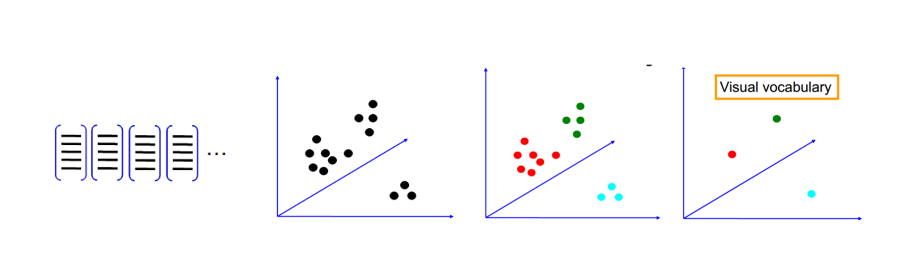
\includegraphics[width=\textwidth]{./project3/bow-step.png}
    \caption{视觉词典建立过程的流程,从左到右依次经过聚类和池化,得到视觉词典。}
\end{figure}

\subsubsection{分类}
分类识别是整个流程的最后一步。在对训练和测试样本都进行表达之后,需要对影像进行监督分类。由于影像的特征维度一般都比较高,并且训练数据规模通常要比测试数据小,所以考虑选用支持向量机(Support Vector Machine, SVM)作为分类器。 

在使用SVM时,核函数的选取是十分重要的,常用的核函数包括:线性核,多项式核,高斯核等。不过在场景识别问题上,最有效的核函数是直方交叉核(Histogram Intersection Kernel, HIK)。

\subsection{实验结果}
\begin{figure}[h]
    \centering
    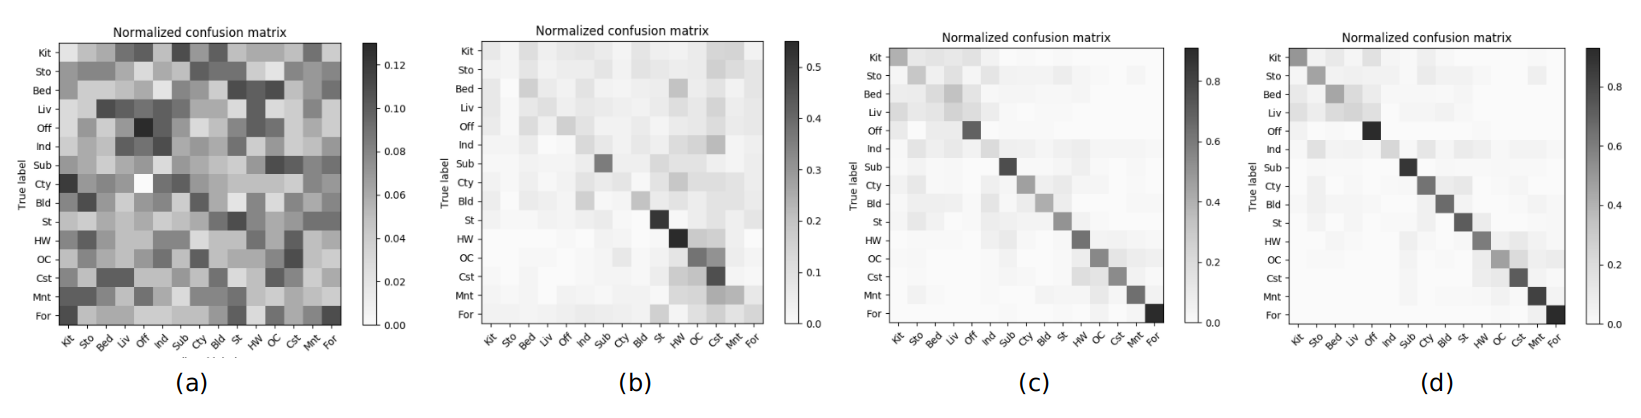
\includegraphics[width=\textwidth]{./project3/result.png}
    \caption{混淆矩阵。(a)使用随机选择进行分类的结果;(b)使用小图像特征进行分类的结果;(c)使用SIFT+KNN进行分类的结果;(d)使用SIFT+SVM进行分类的结果。}
\end{figure}

\begin{table}[ht]
    \centering
    \begin{tabular}{ccccc}
        \toprule
        & Random & Tiny Images & SIFT+KNN & SIFT+SVM\\
        \midrule
        准确率(\%) & 7.5 & 20.2 & 52.8 & 65.4 \\
        \bottomrule
    \end{tabular}
    \caption{使用不同算法的分类准确率}
\end{table}

\subsection{核心代码}
\begin{lstlisting}
from PIL import Image
import numpy as np
from scipy.spatial import distance
import pickle
import scipy.spatial.distance as distance
from cyvlfeat.sift.dsift import dsift
from time import time
import pdb

def get_bags_of_sifts(image_paths):
    f = open('vocab.pkl', 'rb')
    voc = pickle.load(f)
    voc_size = len(voc)
    len_img = len(image_paths)
    image_feats = np.zeros((len_img, voc_size))
    
    for idx, path in enumerate(image_paths):
        img = np.asarray(Image.open(path),dtype = 'float32')
        frames, descriptors = dsift(img, step=[5,5], fast=True)
        d = distance.cdist(voc, descriptors, 'euclidean')
        dist = np.argmin(d, axis = 0)
        histo, bins = np.histogram(dist, range(voc_size+1))
        norm = np.linalg.norm(histo)
        if norm == 0:
            image_feats[idx, :] = histo
        else:
            image_feats[idx, :] = histo/norm
    return image_feats


def build_vocabulary(image_paths, vocab_size):
    bag_of_features = []
    print("Extract SIFT features")
    #pdb.set_trace()
    for path in image_paths:
        img = np.asarray(Image.open(path), dtype = 'float32')
        frames, descriptors = dsift(img, step = [5,5], fast = True)
        bag_of_features.append(descriptors)
    bag_of_features = np.concatenate(bag_of_features, axis = 0).astype('float32')
    #pdb.set_trace()
    print("Compute vocab")
    start_time = time()
    vocab = kmeans(bag_of_features, vocab_size, initialization = "PLUSPLUS")
    end_time = time()
    print("It takes ", (start_time - end_time), " to compute vocab.")

    return vocab

    def get_tiny_images(image_paths):

    '''
    Input : 
        image_paths: a list(N) of string where where each string is an image 
        path on the filesystem.
    Output :
        tiny image features : (N, d) matrix of resized and then vectorized tiny
        images. E.g. if the images are resized to 16x16, d would equal 256.
    '''
    
    width = height = 16
    
    tiny_images = np.zeros((len(image_paths), width * height), dtype = 'float32')
    
    for num in range(len(image_paths)):
        img = Image.open(image_paths[num])
        img_resize = np.asarray(img.resize((width, height), Image.ANTIALIAS), dtype='float32')
        img_resize = img_resize.flatten()
        img_tiny = (img_resize-np.mean(img_resize))/np.std(img_resize)
        tiny_images[num, :] = img_tiny
    return tiny_images

    def svm_classify(train_image_feats, train_labels, test_image_feats):
    
    clf = LinearSVC()
    #C=0.005,random_state=0, tol=1e-5
    #This for RBF kernel
    #clf = SVC(kernel = 'rbf', random_state=0, gamma = 0.2, C=10)
    clf.fit(train_image_feats, train_labels)
    pred_label = clf.predict(test_image_feats)
    
    sc = cross_val_score(clf, train_image_feats, train_labels)
    print ('Validation Score:',sc.mean())
    return pred_label
    
\end{lstlisting}

\end{document}